\begin{figure}[ht]
    \centering

    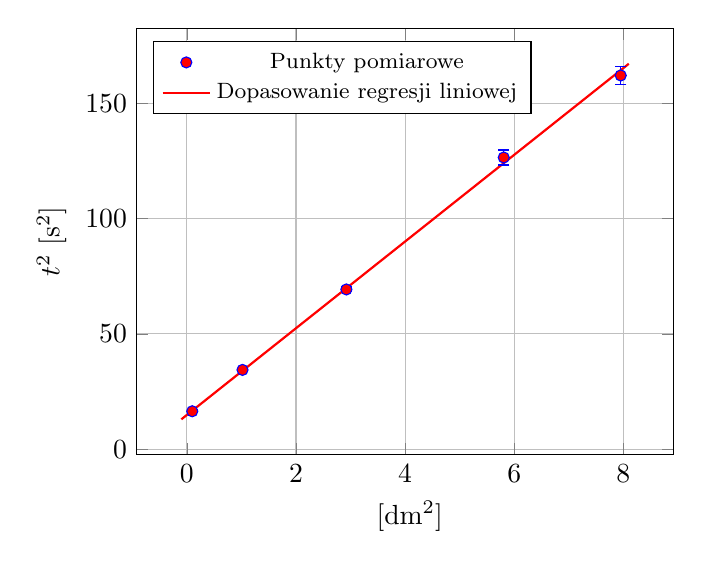
\begin{tikzpicture}
        \begin{axis}[
            width=8.4cm, height=7cm,
            xlabel={$\dwSq~[\mathrm{dm^2}]$},
            ylabel={$t^2~[\mathrm{s}^2]$},
            legend pos=north west,
            grid=major,
            legend style={font=\footnotesize}
        ]

        \addlegendimage{only marks, mark=*, blue, mark options={fill=red}, error bars/.cd, y dir=both, y explicit}
        \addlegendentry{Punkty pomiarowe}
        
        \addlegendimage{no markers, red, thick}
        \addlegendentry{Dopasowanie regresji liniowej}
        
        \def\slope{18.7965233}
        \def\intercept{14.8481}
        
        \addplot [red, thick, domain=-0.1:8.1, forget plot] {\slope*x + \intercept};
        \addlegendentry{Dopasowanie regresji liniowej}
    
        \addplot+[
            only marks,
            mark=*,
            blue,
            mark options={fill=red},
            forget plot,
            error bars/.cd,
            y dir=both,
            y explicit,
        ] table [x=x, y=y, y error=err] {
            x           y               err
            7.9524      162.027441      4.061729736
            0.099225    16.45356969     0.5661758554
            2.9241      69.26899984     1.080984169
            1.0201      34.39001449     0.5575028803
            5.8081      126.4680176     3.259685309
        };
        \addlegendentry{Punkty pomiarowe}
    
        \end{axis}
    \end{tikzpicture}

    \caption{
        Dane pomiarowe dla Zależności II wraz z dopasowaniem regresji liniowej: $t^2(\dwSq) = a~\dwSq + b$. Niepewności $t^2$ są ledwo widoczne na wykresie, niepewności $\dwSq$ są na tyle małe, że nie widać ich wcale.
    }
    \label{img:regresja-ii-wykres}
\end{figure}
